%%%%%%%%%%%%%%%%%%%%%%%%%%%%%%%%%%%%%%%%%
% University/School Laboratory Report
% LaTeX Template
% Version 3.1 (25/3/14)
%
% This template has been downloaded from:
% http://www.LaTeXTemplates.com
%
% Original author:
% Linux and Unix Users Group at Virginia Tech Wiki 
% (https://vtluug.org/wiki/Example_LaTeX_chem_lab_report)
%
% License:
% CC BY-NC-SA 3.0 (http://creativecommons.org/licenses/by-nc-sa/3.0/)
%
%%%%%%%%%%%%%%%%%%%%%%%%%%%%%%%%%%%%%%%%%

%----------------------------------------------------------------------------------------
%	PACKAGES AND DOCUMENT CONFIGURATIONS
%----------------------------------------------------------------------------------------

\documentclass{article}

\usepackage[version=3]{mhchem} % Package for chemical equation typesetting
%\usepackage{siunitx} % Provides the \SI{}{} and \si{} command for typesetting SI units
\usepackage{graphicx} % Required for the inclusion of images
\usepackage{natbib} % Required to change bibliography style to APA
\usepackage{amsmath} % Required for some math elements 
\usepackage{hyperref}
 \usepackage{pdflscape}
\usepackage[a4paper,margin=0.5in]{geometry}
\setlength\parindent{0pt} % Removes all indentation from paragraphs

\renewcommand{\labelenumi}{\alph{enumi}.} % Make numbering in the enumerate environment by letter rather than number (e.g. section 6)

%\usepackage{times} % Uncomment to use the Times New Roman font

%----------------------------------------------------------------------------------------
%	DOCUMENT INFORMATION
%----------------------------------------------------------------------------------------

\title{Gate Detection} % Title

\author{Philipp \textsc{Duernay}} % Author name

\date{\today} % Date for the report

\begin{document}
\maketitle
% If you wish to include an abstract, uncomment the lines below
% \begin{abstract}
% Abstract text
% \end{abstract}

%----------------------------------------------------------------------------------------
%	SECTION 1
%----------------------------------------------------------------------------------------

\section{Recap}
In the last meeting from 22.04.2018 several next steps were defined:
\begin{itemize}
	\item Investigate further what makes YoloV2 perform better.
	\item Refine Architecture.
	\item Implement GateNet on JeVois.
	\item Do some speed measurements.
\end{itemize}


\section{Implementation on JeVois}

It is possible to run a tensorflow lite model on the JeVois. Tensorflow lite is a library that optimizes model inference for mobile devices. Hence, by using this library we could already make full use of the GPU without doing a lot of manual work. It is "only" required to transform the model into tflite format. Unfortunately, the conversion throws an error when converting the "Batch Normalization" layer. Several other people met this problem before and discuss it on GitHub, so we can hope there will be a fix soon. If the problem is not fixed soon we can still use darknet a c-framework for neural nets by the yolo-people. However, that would require more manual programming.

\section{Experiments}

We assume due to the simplicity of the objects we want to detect it should be possible to use a much simpler network than YoloV2. Hence, we evaluate additional architectures in terms of detection performance and number of parameters. \autoref{tab:models} summarizes the evaluated architectures. Result plots can be found on the following pages.

As the final implementation should run on a mobile device, we are also interested in inference speed. Hence, we evaluate each model in terms of speed on a PASCAL GPU with 12GB. The presented results are the average over 500 images.

Multiple parameters are evaluated:
\begin{itemize}
	\item \textbf{depth} (amount of layers). Typically more layers improve the performance as models can learn deeper semantic representations. However, in our case the object consist of quite simple shapes, not so many deep layers should be required.
	
	We have two examples where the only thing that changes is the number of layers. These are from gatev8 to gatev11 and gatev10 to gatev17. In both cases the performance even drops. Hence, simply making the model deeper does not seem to increase performance. Although the best performing model is still the deepest one.
	
	As expected the inference speed increases when adding more layers. Still the fastest model is gatev12 with 7 layers. Making the network even smaller requires increasing the kernels of the filters which leads to more computations.
	
	\item \textbf{kernel size}. In the last report we saw how a too shallow model did not achieve great performance as the receptive field of the predictor layers was too small. Instead of making the model deeper we can also increase the kernel size of the filters.
	
	gatev14 is an example for a very shallow network with large kernels. However, it does not perform well compared to other networks. Despite having less layers it does not get faster as the large kernels are heavier to compute.
	
	In gatev9 and gatev10 we see a network similar to gatev8 but with less layers and larger kernels. Both networks improve towards gatev8. Gatev10 has 3x3 convolutions in the higher layers. Thus it seems increasing the kernel sizes in the lower layers benefits the model.
	
	
	\item \textbf{pooling}. Our object consists largely of background. Hence, we assume larger pooling should not hurt performance but reduce model size.
	
	We see two examples where only the pooling changes. That is from gatev8 to gatev13 and gatev10 to gatev16. In the first case the performance stays the same, while in the second case the performance detoriates a bit. In both cases we see a boost in speed.
	
	
	\item \textbf{width} (amount of filter maps per layer). With more filters, each filter can specialize for certain input patterns. Wider networks are computationally cheaper than deeper networks as the forward pass across multiple filter maps can be computed in parallel.
	
	In the last report we saw already how the width can drastically be reduced. E.g. Gatev8 is essentially a thinner version of TinyYolo. We see a huge drop in weights an increase in speed and only a small loss in performance.
	
	Generally we don't seem to require a wide network. E.g. gatev20 increases the amount of filters towards gatev19 and the performance as well as the speed gets worse. 

\end{itemize}

An additional experiment was gatev15. Inspired by MobileNet, we use depthwise seperable convolutions instead of standard convolutions. This should make the model smaller and faster, while maintaining performance. In our experiment we see quite a big drop in performance without really increasing speed. The fastest model is still a model with standard convolutions.

\begin{figure}
	\centering
	\begin{minipage}{0.45\linewidth}
		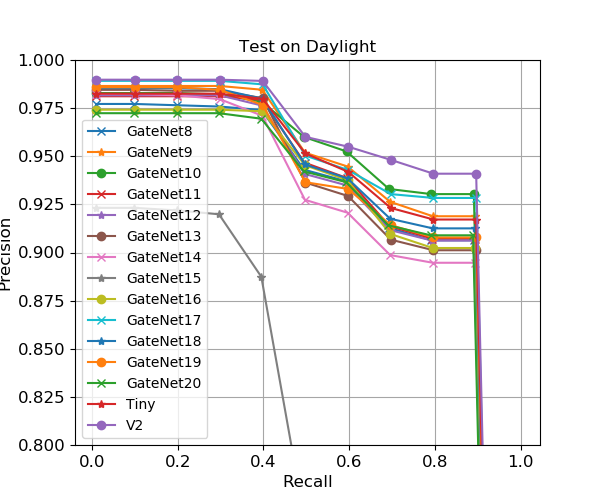
\includegraphics[width=\linewidth]{fig/test_daylight}
	\end{minipage}
	\begin{minipage}{0.45\linewidth}
		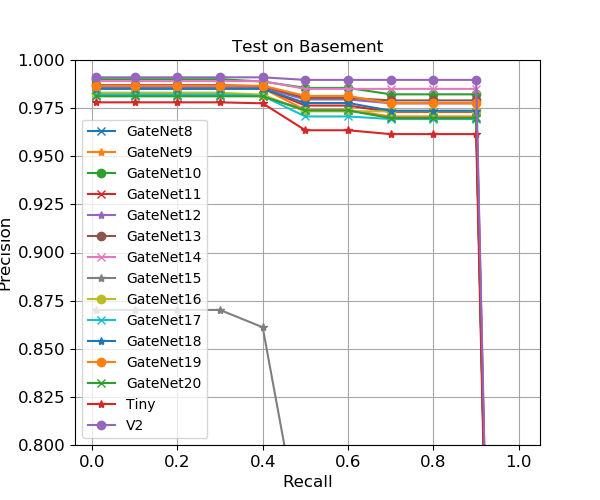
\includegraphics[width=\linewidth]{fig/test_basement}
	\end{minipage}
	\caption{Precision-Recall for all models.}
\end{figure}

\begin{figure}
	\centering
	\begin{minipage}{0.45\linewidth}
		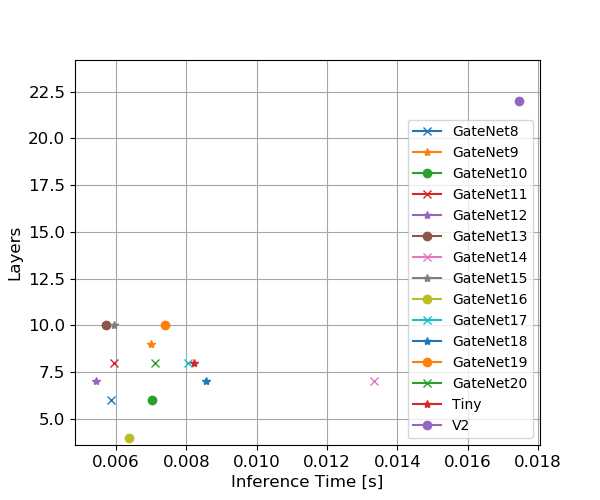
\includegraphics[width=\linewidth]{fig/layers_speed}
		\caption{Depth vs speed}
	\end{minipage}
	\begin{minipage}{0.45\linewidth}
		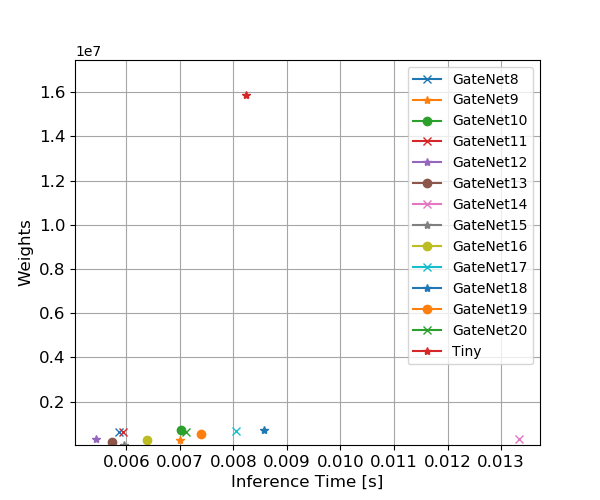
\includegraphics[width=\linewidth]{fig/weights_speed}
		\caption{Modelsize vs speed}
	\end{minipage}
	
\end{figure}

\begin{figure}
	\centering
	\begin{minipage}{0.45\linewidth}
		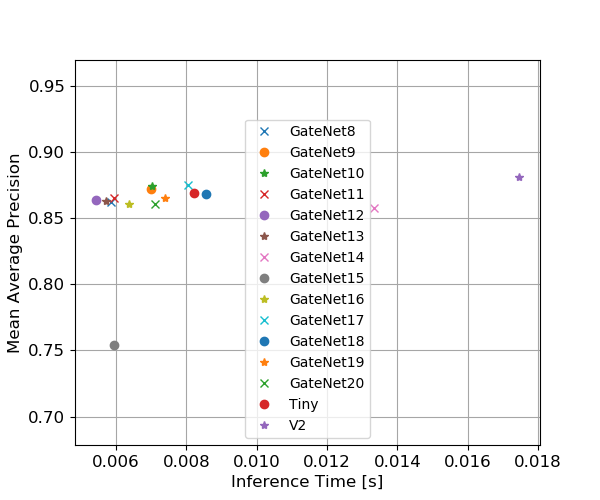
\includegraphics[width=\linewidth]{fig/perf_speed}
		\caption{Performance vs speed}
	\end{minipage}
	\begin{minipage}{0.45\linewidth}
		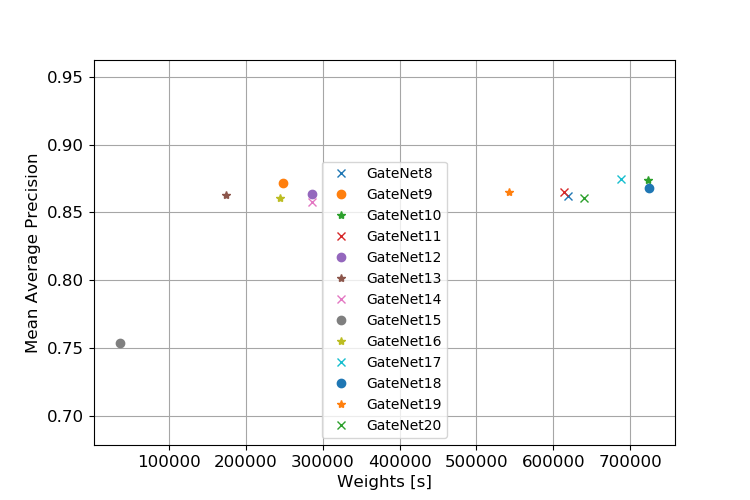
\includegraphics[width=\linewidth]{fig/perf_weights}
		\caption{Performance vs speed}
	\end{minipage}
	
\end{figure}

\begin{figure}
	\centering
	\begin{minipage}{0.45\linewidth}
		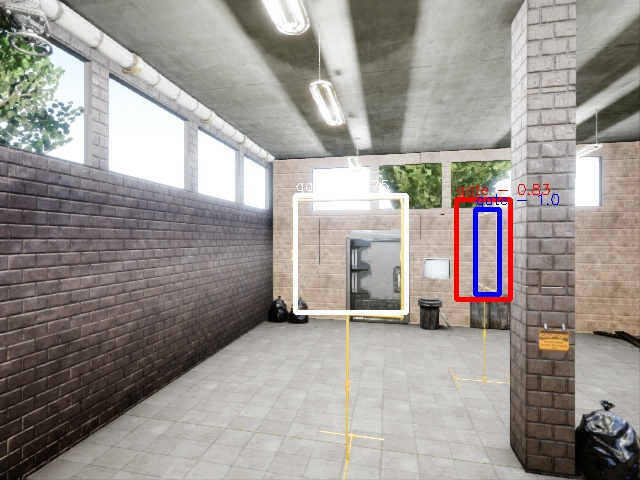
\includegraphics[width=\linewidth]{fig/example1_gate}
	\end{minipage}
	\begin{minipage}{0.45\linewidth}
		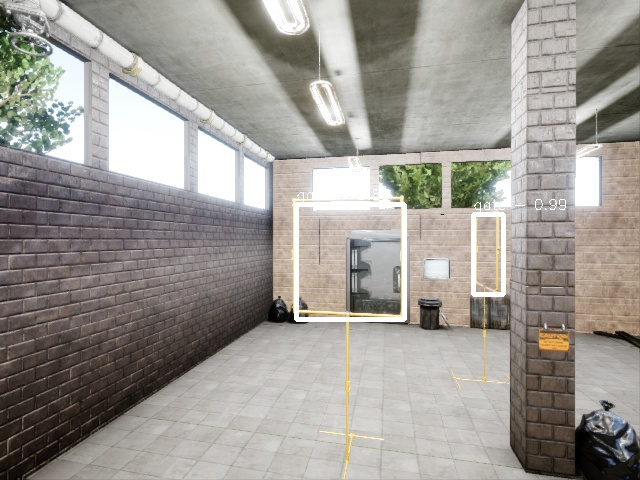
\includegraphics[width=\linewidth]{fig/example1_yolo}
	\end{minipage}
	
	\begin{minipage}{0.45\linewidth}
		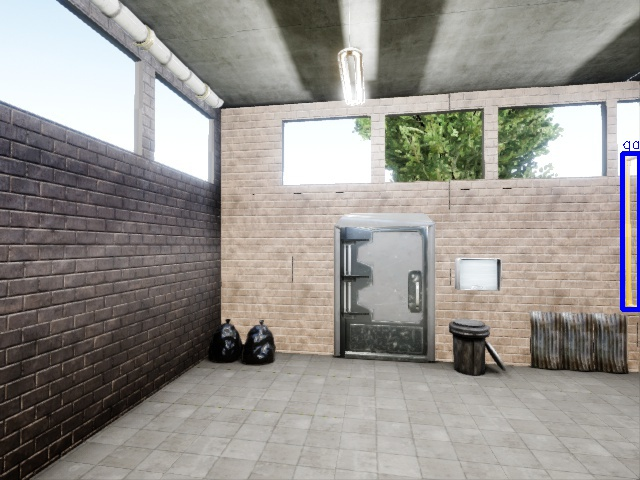
\includegraphics[width=\linewidth]{fig/example2_gate}
	\end{minipage}
	\begin{minipage}{0.45\linewidth}
		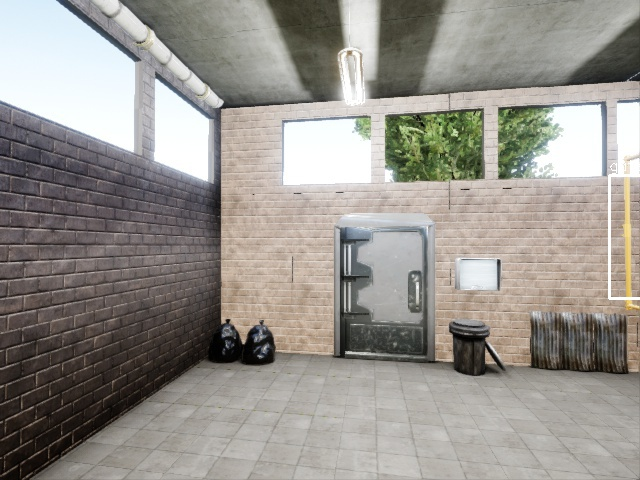
\includegraphics[width=\linewidth]{fig/example2_yolo}
	\end{minipage}
	\caption{Two examples where yolo (right) outperforms gatenet. Wee see false negatives in blue, true positives in white, false positives in red.}
\end{figure}


\section{Conclusion}

\begin{itemize}
	
	\item The fastest model is not necessarily the smallest one. E.g. gatev15 and gatev14 are quite small but slower than a lot of other models.
	
	\item The boost in speed is not as big as expected. Despite reducing the model size significantly the inference time only reduced by ~2ms.
	
	\item Early, large pooling increases speed significantly but can also hurt performance
	
	\item Lower order layers benefit from larger kernels
	
	\item The overall network benefits (in terms of performance and speed) from depth rather than larger kernels
	
	\item We could reduce the modelsize while keeping the same performance level. However, the best model is still YoloV2.
	
	\item Yolo seems to perform better on the very steep angles/difficult objects
\end{itemize}

\section{Next Step}

\begin{itemize}
	\item Finish implementation on JeVois to see "real" performance.
	\item Investigate more measures to increase speed
\end{itemize}


\newpage
\begin{landscape}


\begin{table}[]
	\small
	\centering
	\caption{Summary}
	\label{tab:models}
	\begin{tabular}{|l|p{2cm}|l|l|l|l|l|l|l|l|l|l|l|l|l|l|l|l|l|l|}
		\hline
		Name & Comment                                                           & mAP   & T{[}ms{]} & n\_weights & 1      &      & 2        &      & 4         &      & 5         &      & 6       &      & 7       &      & 8        & 9       & 10     \\ \hline
		v8   & best model last time                                              & 0.862 & 5.85      & 619529     & 16C3x3 & P2x2 & 32C3x3   & P2x2 & 64C3x3    & P2x2 & 64C3x3    & P2x2 & 64C3x3  & P2x2 & 64C3x3  &      & 64C3x3   & 64C3x3  &        \\ \hline
		v9   & more shallow larger kernels                                       & 0.871 & 7.00      & 248265     & 16C6x6 & P2x2 & 64C6x6   & P2x2 & 64C6x6    & P2x2 & 64C6x6    & P2x2 & 64C9x9  &      &         &      &          &         &        \\ \hline
		v10  & like v9 but last layer with smaller kernels                       & 0.874 & 7.02      & 723417     & 16C6x6 & P2x2 & 64C6x6   & P2x2 & 64C6x6    & P2x2 & 64C6x6    & P2x2 & 64C3x3  &      & 64C3x3  &      & 64C3x3   &         &        \\ \hline
		v11  & like v8 but deeper                                                & 0.865 & 5.94      & 613337     & 16C3x3 & P2x2 & 32C3x3   & P2x2 & 64C3x3    & P2x2 & 64C3x3    & P2x2 & 64C3x3  & P2x2 & 64C3x3  &      & 64C3x3   & 64C3x3  & 64C3x3 \\ \hline
		v12  & like v8 but 4x4 pool, less layers                                 & 0.863 & 5.43      & 285385     & 16C3x3 & P2x2 & 32C3x3   & P4x4 & 64C3x3    & P4x4 & 64C3x3    &      & 64C3x3  &      & 64C3x3  &      &          &         &        \\ \hline
		v13  & like v8 but 4x4                                                   & 0.862 & 5.73      & 174025     & 16C3x3 & P2x2 & 32C3x3   & P4x4 & 64C3x3    & P4x4 & 64C3x3    &      & 64C3x3  &      & 64C3x3  &      & 64C3x3   &         &        \\ \hline
		v14  & shallow but large kernels                                         & 0.857 & 13.3      & 285385     & 32C6x6 &      & 64C12x12 &      & 128C12x12 &      & 256C12x12 &      &         &      &         &      &          &         &        \\ \hline
		v15  & like v10 but depthwise seperable conv                             & 0.753 & 5.55      & 36341      & 16C6x6 & P2x2 & 32C6x6   & P2x2 & 64DC6x6   & P2x2 & 64DC6x6   & P2x2 & 64C3x3  &      & 64C3x3  &      & 64DC3x3  &         &        \\ \hline
		v16  & like v10 but 4x4 pooling                                          & 0.860 & 6.38      & 244441     & 16C6x6 & P2x2 & 32C6x6   & P4x4 & 64C6x6    & P4x4 & 64C6x6    &      & 64C3x3  &      & 64C3x3  &      & 64C3x3   &         &        \\ \hline
		v17  & \begin{tabular}[c]{@{}l@{}}like v10\\ but deeper\end{tabular}     & 0.874 & 8.04      & 687577     & 16C6x6 & P2x2 & 32C6x6   & P2x2 & 64C6x6    & P2x2 & 64C6x6    & P2x2 & 64C3x3  & P2x2 & 64C3x3  &      & 64C3x3   & 64C3x3  & 64C3x3 \\ \hline
		v18  & \begin{tabular}[c]{@{}l@{}}like v10\\ pooling higher\end{tabular} & 0.867 & 8.56      & 723929     & 16C6x6 & P2x2 & 32C6x6   & P2x2 & 64C6x6    &      & 64C6x6    & P2x2 & 64C6x6  & P2x2 & 64C6x6  & P2x2 & 64C3x3   &         &        \\ \hline
		v19  & like v18 but smaller kernel                                       & 0.865 & 7.38      & 542921     & 16C3x3 & P2x2 & 32C3x3   & P2x2 & 64C3x3    &      & 64C3x3    & P2x2 & 64C3x3  & P2x2 & 64C3x3  & P2x2 & 64C3x3   &         &        \\ \hline
		v20  & like v19 but more filters                                         & 0.860 & 7.11      & 640073     & 16C3x3 & P2x2 & 64C3x3   & P2x2 & 128C3x3   & P2x2 & 64C3x3    & P2x2 & 64C3x3  &      & 64C3x3  &      & 64C3x3   &         &        \\ \hline
		Yolo &                                                                   & 0.869 & 8.2       & 15867885   & 16C3x3 & P2x2 & 32C3x3   & P2x2 & 64C3x3    &      & 128C3x3   & P2x2 & 256C3x3 & P2x2 & 512C3x3 & P2x2 & 1024C3x3 &         &        \\ \hline
		Yolo &                                                                   & 0.881 & 17.45     & 50676436   & 32C3x3 & P2x2 & 64C3x3   & P2x2 & 128C3x3   &      & 64C3x3    &      & 128C3x3 & P2x2 & 256C3x3 &      & 128C3x3  & 256C3x3 & P2x2   \\ \hline
	\end{tabular}
\end{table}
\end{landscape}


%----------------------------------------------------------------------------------------


%----------------------------------------------------------------------------------------


\end{document}\grid
